\documentclass[a4paper,12pt]{article}
\usepackage{graphicx, float, enumerate, parskip}
\usepackage{amsmath, amssymb, amsthm}
\theoremstyle{definition}
\newtheorem{definition}{Definisi}[section]
\newtheorem{theorem}{Teorema}[section]
\newtheorem{example}{Contoh}[section]
\usepackage{listings, fancyvrb, spverbatim, xcolor}
\lstset{% setup listings
    language=R,% set programming language
    frame=tb,
    basicstyle=\ttfamily\small,% basic font style
    keywordstyle=\color{blue},% keyword style
    commentstyle=\color{gray},% comment style
    breaklines=true,% automatic line breaking
    fancyvrb=true,% verbatim code is typset by listings
}
\usepackage[
    backend=biber,
    style=bwl-FU,
    sorting=nyt,
    maxbibnames=99,
    natbib=true,
]
{biblatex}
\addbibresource{DPustaka.bib}

%% ---------------------------
\begin{document}
    \title{Pembangkitan Proses Random}
    \author{Gustian\\
            Kuncoro Adi W}
\date{\today}

\begin{titlepage}
    \maketitle
\end{titlepage}


\section{Proses Stokastik} 
Proses stokastik adalah kumpulan $\left \{X\left ( t \right ):t \in T \right \}$ dari variabel acak diindeks oleh set T, yang biasanya mewakili waktu. Set indeks T dapat berupa diskrit atau kontinu. Himpunan nilai yang mungkin diambil $X\left ( t \right )$ adalah keadaan ruang, yang juga dapat diskrit atau kontinu. Ross (2014) memberikan pengantar yang baik untuk proses stokastik, dan termasuk bab mengenai simulasi.

Proses penghitungan mencatat jumlah kejadian atau kemunculan yang terjadi waktu $\textit{t}$. Proses penghitungan memiliki $\textit{kenaikan independen}$ apabila jumlah kemunculan dalam interval waktu terpisah adalah independen. Proses penghitungan memiliki $\textit{peningkatan stasioner}$ jika jumlah peristiwa yang terjadi dalam suatu interval hanya bergantung pada panjang intervalnya. Contohnya adalah proses Poisson.

Untuk mempelajari proses penghitungan melalui simulasi, kita dapat menghasilkan realisasi dari proses yang merekam kejadian untuk periode waktu yang terbatas. Himpunan waktu kedatangan secara berturut-turut mencatat hasil dan menentukan keadaan $X\left ( t \right )$ setiap saat $\left ( t \right )$. Dalam sebuah simulasi, urutan waktu kedatangan harus terbatas. Salah satu metode simulasi untuk proses penghitungan adalah dengan memilih interval waktu yang cukup panjang dan membangkitkan waktu kedatangan atau waktu antar kedatangan dalam interval tersebut.

\subsection{Proses Poisson} 
Proses Poisson homogen $\{N(t), t \geq 0\}$ dengan rate $\lambda$ yang merupakan proses perhitungan, dengan independen inkremen, sehingga $N(0) = 0$.

\begin{equation} \label{S1}
    P(N(s+t)-N(s) = n) = \frac{e^{\lambda t} (\lambda t)^n}{n!},\ \ n \geq 0, t, s > 0.
\end{equation}

Dengan demikian, proses Poisson Homogen memiliki inkremen stasioner dengan jumlah kejadian $N(t)$ dalam $[0, t]$ memiliki distribusi Poisson $\lambda t$. Jika $T_1$ adalah waktu kedatangan pertama, 

\begin{equation*}
    P(T_1 > t) = P(N(t) = 0) = e^{- \lambda t}, \ \ t \geq 0,
\end{equation*}

jadi $T_1$ berdistribusi secara ekponensial dengan rate $\lambda$. Waktu antara kedatangan $T_1, T_2, ...$ merupakan waktu antara kedatangan yang berturut-turut. Waktu kedatangan merupakan eksponensial iid dengan rate $\lambda$, yang mengikuti persamaan \ref{S1} dan sifat yang berdistribusi eksponensial.

Salah satu metode untuk mensimulasikan proses Poisson adalah dengan menghasilkan waktu antara kedatangan. Waktu ke-$n$ adalah jumlah $S_n = T_1 + ... + T_n$ (waktu tunggu sampai kedatangan ke-$n$). Urutan waktu antara kedatangan $\{ T_n \}^\infty _{n=1}$ atau urutan waktu kedatangan $\{ S_n \}^\infty _{n=1}$ yang merupakan realisasi dari proses tersebut. Jadi, realisasi tersebut merupakan urutan takhingga, yang bukan angka tunggal. Dalam simulasi, urutan waktu antara kedatangan $\{T_n\}^N _{n=1}$ atau waktu kedatangan $\{S_n\}^N _{n=1}$ adalah realisasi simulasi dari proses pada interval $[0, S_N)$.

Metode lain untuk mensimulasikan proses Poisson adalah dengan menggunakan fakta bahwa distribusi kondisional dari waktu kedatangan (tidak terurut) dengan diberikan $N(t)=n$ sama dengan sampel acak berukuran $n$ dari distribusi Uniform $(0, t)$. 

Keadaan proses pada waktu tertentu $t$ sama dengan jumlah kedatangan di $[0, t]$, yang merupakan jumlah min $(k : S_k > t) - 1$. Yaitu, $N(t) = n - 1$, dimana $S_n$ merupakan waktu kedatangan terkecil yang melebihi $t$.

\textbf{Algoritma untuk mensimulasikan proses Poison homogen pada interval $[0, t_0]$ dengan membangkitkan waktu antara kedatangan.} 
\begin{enumerate}
    \item Tetapkan $S_1 = 0$.
    \item Untuk $j = 1, 2, ...$ ketika $S_j \leq t_0$:
        \begin{enumerate}
            \item Menghasilkan $T_j \sim$ Exp $(\lambda)$.
            \item Atur $S_j = T_1 + ... + T_j$.
        \end{enumerate}
    \item $N(t_0) =$ min$_j(S_j > t_0) - 1$. 
\end{enumerate}

Persamaan diatas tidak efisien untuk diterapkan pada R dengan pengulangan \texttt{for}. Persamaan tersebut perlu diterjemahkan ke dalam operasi vektor, seperti contoh berikut.

\begin{example} (Proses Poisson). \label{C1}\\
Contoh ini mengilustrasikan pendekatan sederhana untuk menyimulasikan proses Poisson dengan rate $\lambda$. Misalkan kita mempunyai $N(3)$, dengan jumlah kedatangan $[3, 0]$. Hasilkan iid eksponensial waktu $T_i$ dengan rate $\lambda$ dan temukan indeks $n$ di mana jumlah kumulatif $S_n = T_1 + ... + T_n$ pertama melebihi 3. Maka jumlah kedatangan di $[0, 3]$ adalah $n-1$. Dengan rata-rata jumlah adalah $E[N(3)] = 3\lambda$.

    \begin{lstlisting}
    lambda <- 2
    t0 <- 3
    Tn <- rexp(100, lambda)   #waktu antara kedatangan
    Sn <- cumsum(Tn)          #waktu kedatangan
    n <- min(which(Sc > t0))  #interval+1 dalam [0, t0]
    \end{lstlisting}

Hasil dari dua run ditunjukan di bawah ini.

    \begin{lstlisting}
    > n-1
    [1] 8
    > round(Sn[1:n], 4)
    [1] 1.2217 1.3307 1.3479 1.4639 1.9631 2.0971
        2.3249 2.3409 3.9814
        
    > n-1
    [1] 5
    > round(Sn[1:n], 4)
    [1] 0.4206 0.8620 1.0055 1.6187 2.6418 3.4739
    \end{lstlisting}

Untuk contoh ini, rata-rata nilai simulasi $N(3) = n - 1$ untuk sejumlah besar proses yang mendekati $E[N(30)] = 3\lambda = 6$.

Metode alternatif untuk menghasilkan waktu kedatangan dari proses Poisson berdasarkan fakta dengan mengingat jumlah kedatangan dalam interval $(0, t)$, distribusi bersyarat dari waktu kedatangan tak terurut berdistribusi secara seragam pada $(t, 0)$. Artinya, \textit{diberikan sejumlah kedatangan di} $(0, t)$ \textit{adalah} $n$, waktu kedatangan $S_1, ..., S_n$ didistribusikan secara bersama-sama sebagai sampel acak terurut berukuran $n$ dari distribusi Uniform $(0, t)$.

Menerapkan distribusi bersyarat dari waktu kedatangan, memungkinkan untuk mensimulasi proses Poisson $\lambda$ pada interval $(0, t)$ dengan terlebih dahulu menghasilkan pengamatan acak $n$ dari distribusi Poisson $(\lambda t$, kemudian menghasilkan sampel acak dari $n$ prngamatan Uniform $(0, t)$ dan mengurutkan sampel seragam untuk mendapatkan waktu kedatangan.
\end{example}

\begin{example} (Proses Poisson, lanjutan). \label{C2}\\
Kembali ke contoh \ref{C1}, simulasikan proses Poisson $(\lambda)$ dan temukan $N(3)$, menggunakan distribusi bersyarat dari waktu kedatangan. Sebagai pemeriksa, kita memperkirakan rata-rata dan varian $N(3)$ dari 10.000 replikasi.

    \begin{lstlisting}
    lambda <- 2
    t0 <- 3
    upper <- 100
    pp <- numeric(10000)
    for (i in 1:10000) {
        N <- rpois(1, lambda * upper)
        Un <- runif(N, 0, upper) #waktu kedatangan tidak terurut
        Sn <- sort(Un)           #waktu kedatangan
        n <- min(which(Sn > t0)) #kedatangan+1 dalam [0, t0]
        pp[i] <- n - 1           #kedatangan dalam [0, t0]
        }
    \end{lstlisting}

Alternatif, pengulangan dapat diganti dengan \texttt{replicate}, seperti berikut.

    \begin{lstlisting}
    pp <- replicate(10000, expr = {
        N <- rpois(1, lambda * upper)
        Un <- runif(N, 0, upper) #waktu kedatangan tidak terurut
        Sn <- sort(Un)           #waktu kedatangan
        n <- min(which(Sn > t0)) #kedatangan+1 dalam [0, t0]
        n - 1 })                 #kedatangan dalam [0, t0]
    \end{lstlisting}

Rata-rata dan varian keduanya harus sama dengan $\lambda t = 6$ dalam contoh ini. Dalam rata-rata sampel dan varian sampel dari nilali yang dihasilkan $N(3)$ memang sangat mendekati 6.

    \begin{lstlisting}
    > c(mean(pp), var(pp))
    [1] 5.977100 5.819558
    \end{lstlisting}
    
Dalam beberapa kasus, tidak mungkin ada waktu kedatangan yang dihasilkan yang melebihi waktu ke $t_0 = 3$. Jika hal ini terjadi, maka simulasi harus dilakukan untuk waktu yang lebih lama daripada nilai yang ditentukan pada parameter \texttt{upper}. Oleh karena itu, pada praktiknya, kita harus memilih nilai \texttt{upper} yang sesuai dengan parameter-parameter dari proses tersebut, dan melakukan pemeriksaan kesalahan. Sebagai contoh, jika kita memerlukan $N(t_0)$, maka salah satu pendekatan yang bisa digunakan adalah membungkus langkah \texttt{min(which())} dengan \texttt{try} dan memeriksa apakah hasil dari \texttt{try} adalah bilangan bulat dengan menggunakan fungsi \texttt{is.integer}. Untuk informasi lebih lanjut, Anda dapat melihat topik bantuan yang terkait.

Dalam buku Ross [251], dibahas mengenai efisiensi komputasi dari dua metode yang digunakan pada Contoh \ref{C1} dan \ref{C2} Metode kedua jauh lebih lambat (sekitar 4 atau 5 kali lebih lambat) dibandingkan dengan metode pertama (Contoh \ref{C1}) ketika diimplementasikan dalam R. Generator \texttt{rexp} hampir secepat \texttt{runif}, sedangkan operasi pengurutan menambahkan waktu $O(n \log (n))$. Beberapa peningkatan kinerja mungkin bisa dicapai jika algoritme tersebut diimplementasikan dalam bahasa C dan menggunakan algoritme pengurutan yang lebih cepat untuk nomor seragam.
\end{example}   

\textbf{Proses Poisson Nonhomogen}

Proses perhitungan merupakan Poisson proses dengan fungsi intesnsitas $\lambda (t)$, $t \geq 0$ jika $N(t) = 0$, $N(t)$ mempunyai independen inkremen, dan untuk $h > 0$,
    \begin{equation*}
        P(N(t + h) - N(t) \geq 2) = o(h), {and}
    \end{equation*}
    \begin{equation*}
        P(N(t + h) - N(t) = 1) = \lambda (t)h + o(h)
    \end{equation*}
    
Poisson proses $N(t)$ tidak homogen jika fungsi intensitas $\lambda (t)$ tidak konstan. Proses Poisson nonhomogen memiliki inkremen independen tetapi tidak memiliki inkremen stasioner. Distribusi dari 
    \begin{equation*}
        N(s +t) - N(s)
    \end{equation*}

merupakan Poisson dengan rata-rata $\int_{s}^{s+t} \lambda (y) dy$. Fungsi $m (t) = E[N(t)] = \int_{0}^{t} \lambda (y) dy$ bisa disebut \textit{mean value function} dari proses. Catat bahwa $m(t) = \lambda$ dalam kasus proses Poisson homogen, di mana fungsi intensitas konstan.

Setiap proses Poisson nonhomogen dengan fungsi intensitas terbatas dapat diperoleh dengan sampling waktu proses Poisson homogen. Misalnya  $\lambda(t) \leq \lambda < \infty$ untuk semua $t \geq 0$. Kemudian pengambilan sampel proses Poisson $(\lambda$ sedemikian rupa sehingga peristiwa yang terjadi pada waktu t diterima atau dihitung dengan probabilitas $\lambda (t)/\lambda$ menghasilkan proses yang homogen dengan fungsi intensitas $\lambda (t)$. Untuk melihat ini, misalkan $N(t)$ adalah jumlah kejadian yang diterima dalam $[0, t]$. Maka $N(t)$ berdistribusi Poisson dengan rata-rata
    \begin{equation*}
        E[N(t)] = \lambda \int_{0}^{t} \frac{\lambda (y)}{\lambda} dy = \int_{0}^{t} \lambda (y) dy.
    \end{equation*}

Untuk mensimulasikan proses Poisson nonhomogen pada interval $ [0, t_0]$, cari $\lambda_0 < \infty$ sehingga $\lambda(t) <= \lambda_0$, $0 \leq t \leq t_0$. Kemudian bangkitkan dari proses homogen Poisson $(\lambda_0)$ dengan waktu kedatangan $\{S_j\}$, dan terima setiap kedatangan dengan probabilitas $\lambda (S_j)/\lambda_0$. Langkah-langkah untuk mensimulasikan proses pada interval $[0, t_0)$ adalah sebagai berikut.

\textbf{Algoritma untuk mensimulasikan proses Poisson yang tidak homogen pada interval $[0, t_0]$ dengan pengambilan sampel dari proses Poisson yang homogen.}
\begin{enumerate}
    \item Tetapkan $S_1 = 0$.
    \item Untuk $j = 1, 2, ...$ ketika $S_j \leq t_0$:
        \begin{enumerate}
            \item Hasilkan $T_j \sim $ Exp $(\lambda_0)$ dan tetapkan $S_j = T_1 + ... + T_j$.
            \item Hasilkan $U_j \sim $ Gabungan $(0, 1)$.
            \item Jika $U_j \leq \lambda (S_j)/\lambda_0$ terima (perhitungan) kedatangan dan set $I_j = 1$; sebaliknya $I_j = 0$.
        \end{enumerate}
    \item Berikan waktu kedatangan $I_j = 0$. 
\end{enumerate}

Meskipun algoritma ini cukup sederhana, untuk implementasi di R lebih efisien jika diterjemahkan ke dalam operasi vektor. Ini ditunjukkan pada contoh berikutnya.

\begin{example} \label{C3} (Proses Poisson Nonhomogen)

Simulasikan realisasi dari proses Poisson nonhomogen dengan fungsi intensitas $\lambda (t) = 3 \cos^2 (t)$. Di sini fungsi intensitas dibatasi di atas oleh $\lambda = 3$, sehingga kedatangan ke-$j$ diterima jika $U_j \leq 3 \cos^2 (S_j)/3 = \cos^2 (S_j)$.
    
    \begin{lstlisting}
    lambda <- 3
    upper <- 100
    N <- rpois(1, lambda * upper)
    Tn <- rexp(N, lambda)
    Sn <- cumsum(Tn)
    Un <- runif(N)
    keep <- (Un <= cos(Sn)^2) #indicator, as logical vector
    Sn[keep]    
    \end{lstlisting}

Sekarang, nilai dalam \texttt{Sn[keep]} adalah waktu kedatangan yang dipesan dari proses Poisson yang tidak homogen.

    \begin{lstlisting}
    > round(Sn[keep], 4)
    [1] 0.0237 0.5774 0.5841 0.6885 2.3262
    2.4403 2.9984 3.4317 3.7588 3.9297
    [11] 4.2962 6.2602 6.2862 6.7590 6.8354
    7.0150 7.3517 8.3844 9.4499 9.4646 . . .
    \end{lstlisting}
    
Untuk menentukan keadaan proses pada waktu $t = 2 \pi$, misalnya, lihat entri \texttt{Sn} yang diindeks oleh \texttt{keep}.

    \begin{lstlisting}
    > sum(Sn[keep] <= 2*pi)
    [1] 12
    > table(keep)/N
    keep
    FALSE TRUE
    0.4969325 0.5030675
    \end{lstlisting}
    
Jadi $N(2 \pi) = 12$, dan dalam contoh ini kira-kira 50\% kedatangan dihitung.
\end{example}





\subsection{Proses Renewal} %Kun%
Proses renewal merupakan generalisasi dari proses Poisson. Jika $\left \{ N\left ( t \right ),t\geq 0 \right \}$ adalah proses penghitungan, maka ururtan waktu antar kedatangan tidak negatif $T_1$,$T_2$,... adalah iid (tidak harus berdistribusi eksponensial), maka $\left \{ N\left ( t \right ),t\geq 0 \right \}$ adalah proses renewal. Fungsi $m\left ( t \right )=E\left [ N\left ( t \right ) \right ]$ disebut nilai rata-rata fungsi proses, yang secara unik menentukan distribusi waktu antar kedatangan.

Jika distribusi $F_\Upsilon \left ( t \right )$ dari waktu antar kedatangan antar iid ditentukan, maka sebuah proses renewal dapat disimulasikan dengan menghasilkan urutan waktu antar kedatangan, dengan metode yang mirip dengan Contoh \ref{C1}.

\begin{example} (Proses Renewal). \label{K1C4}
Misalkan waktu antar kedatangan dari Proses renewal memiliki distribusi geometrik dengan probabilitas keberhasilan \textit{p}. (Contoh ini dibahas dalam [251].) Maka waktu antar kedatangan adalah bilangan bulat nonnegatif, dan $S_j=T_1+\cdots +T_j$ memiliki distribusi binomial negatif dengan ukuran parameter \textit{r = j} dan probabilitas \textit{p}. Proses tersebut dapat disimulasikan dengan menghasilkan waktu antar kedatangan geometris dan menghitung waktu kedatangan berturut-turut dengan jumlah kumulatif waktu antar kedatangan.

    \begin{lstlisting}
    t0 <- 5
    Tn <- rgeom(100, prob = .2) #interarrival times
    Sn <- cumsum(Tn)            #arrival times
    n <- min(which(Sn > t0))    #arrivals+1 in [0, t0]
    \end{lstlisting}

Distibusi dari $N(t_0)$ dapat diperkirakan dengan mereplikasi simulasi di atas.

    \begin{lstlisting}
    Nt0 <- replicate(1000, expr = {
        Sn <- cumsum(rgeom(100, prob = .2))
        min(which(Sn > t0)) - 1
        })
    table(Nt0)/1000
    Nt0
        0     1     2     3     4     5    6     7
    0.273 0.316 0.219 0.108 0.053 0.022 0.007 0.002
    \end{lstlisting}

Untuk memperkirakan rata-rata $E[N(t)]$, variasikan waktu $t_0$

    \begin{lstlisting}
    t0 <- seq(0.1, 30, .1)
    mt <- numeric(length(t_0))

    for (i in 1:length(t0)) {
        mt[i] <- mean(replicate(1000,
        {
        Sn <- cumsum(rgeom(100, prob = .2))
        min(which(Sn > t0[i])) - 1
        }))
    }
    plot(t0, mt, type = "l", xlab = "t", ylab = "mean")
    \end{lstlisting}

Mari kita bandingkan dengan proses Poisson homogen, dimana antar kali kedatangan memiliki rata-rata konstan. Di sini kita memiliki $p=0.2$ maka rata-rata antar kali kedatangan adalah $0.8/0.2=4$. Proses Poisson yang memiliki rata-rata waktu antar kedatangan 4 memiliki parameter Poisson $\lambda t = t/4$. Kami menambahkan garis referensi ke plot sesuai dengan rata-rata proses Poisson $\lambda t = t/4$ menggunakan abline(0, .25).
Plotnya ditunjukkan pada Gambar 4.1. Seharusnya tidak mengherankan bahwa rata-rata dari proses renewal sangat dekat dengan $\lambda t$, karena distribusi geometrik adalah analog diskrit dari eksponensial; ia memiliki properti tanpa memori. Itu adalah, jika $X \sim Geometrik(p)$, maka untuk semua $j, k = 0, 1, 2, ...$

$P(X>j+k|X>j)=\frac{(1-p)^{j+k}}{(1-p)^{j}}=(1-p)^{k}=P(X>k)$

\end{example}





\begin{figure}
    \centering
    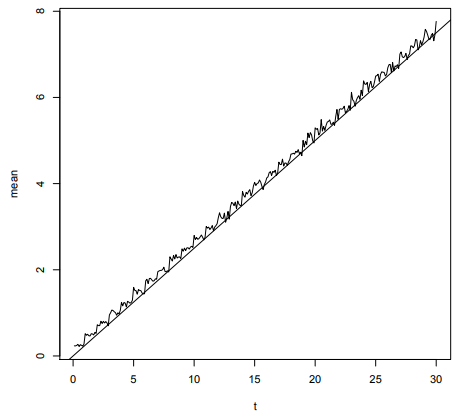
\includegraphics[width=9cm]{gb/K1G1.png}
    \caption{Urutan sarana sampel dari proses pembaharuan yang disimulasikan dalam Contoh \ref{K1C4}. Garis referensi sesuai dengan rata-rata $\lambda t = t/4$ dari proses Poisson yang homogen.}
    \label{K1G1}
\end{figure}


\subsection{Random Walk Simetris}
Misalkan $X_1, X_2, ...$ merupakan barisan variabel acak iid dengan distribusi probabilitas $P(X_i = 1) = P(X_i = -1) = 1/2$. Tentukan jumlah parsial $S_n = \sum_{i=1}^{n} X_i$. Proses $\{S_n, n \geq 0\}$ disebut \textit{random walk simetris}. Sebagai contoh, jika seorang penjudi bertaruh \$1 pada percobaan melempar koin berulang kali, maka $S_n$ menyatakan keuntungan/kerugian setelah $n$ lemparan.



\begin{example} \label{K1C5} (Plot realisasi sebagian dari jalan acak).

Sangat sederhana untuk menghasilkan proses random walk simetris dalam rentang waktu singkat.

    \begin{lstlisting}
    n <- 400
    incr <- sample(c(-1, 1), size = n, replace = TRUE)
    S <- as.integer(c(0, cumsum(incr)))
    plot(0:n, S, type = "l", main = "", xlab = "i")
    \end{lstlisting}
    
Realisasi parsial dari proses random walk simetris yang dimulai dari $S_n = 0$ ditunjukkan pada Gambar \ref{K1G2}. Proses telah kembali ke 0 beberapa kali dalam waktu $[1, 400]$.

    \begin{lstlisting}
    > which(S == 0)
    [1] 1 3 27 29 31 37 41 95 225 229 233 237 239 241
    \end{lstlisting}
    
    

\begin{figure}[H]
    \centering
    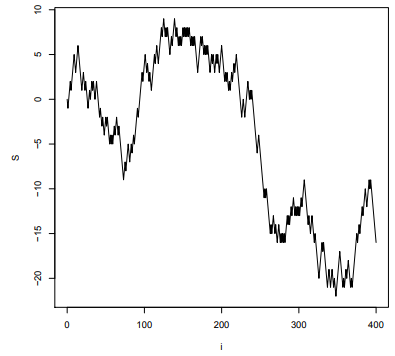
\includegraphics[height=9cm]{gb/K1G2.png}
    \caption{Realisasi parsial dari jalan acak simetris pada Contoh \ref{K1C5}}
    \label{K1G2}
\end{figure}

Nilai $S_n$ dapat ditentukan dengan random walk parsial yang dimulai pada waktu terakhir proses kembali ke 0.

Jika keadaan random walk simetris $S_n$ pada waktu $n$ diperlukan, tetapi bukan riwayat hingga waktu $n$, maka untuk $n$ yang besar mungkin akan lebih efisien untuk membangkitkan $S_n$ sebagai berikut.

Asumsikan bahwa $S_0 = 0$ adalah keadaan awal dari proses. Jika proses telah kembali ke keadaan sebelum waktu $n$, maka untuk menghasilkan $S_n$ kita dapat mengabaikan riwayat masa lalu hingga waktu proses terakhir mencapai $0$. Misalkan $T$ adalah waktu hingga kembalinya yang pertama ke asal. Kemudian untuk menghasilkan $S_n$, seseorang dapat menyederhanakan masalah dengan terlebih dahulu membangkitkan waktu tunggu $T$ hingga total waktu terlebih dahulu melebihi $n$. Kemudian mulai dari pengembalian terakhir ke asal sebelum waktu $n$, hasilkan kenaikan $X_i$ dan jumlahkan.

\textbf{Algoritma untuk mensimulasikan keadaan $S_n$ dari jalan acak simetris}

Algoritma berikut diadaptasi dari [72, XIV.6].

Biarkan $W_j$ menjadi waktu tunggu sampai $j$ kembali ke asal.

\begin{enumerate}
    \item Tetapkan $W_1 = 0$.
    \item Untuk $j = 1, 2, ...$ ketika $W_j \leq n:$
        \begin{enumerate}
            \item Hasilkan $T_j$ acak dari distribusi waktu hingga pengembalian pertama ke 0.
            \item Tetapkan $W_j = T_1 + ... + T_j$.
        \end{enumerate}
    \item Tetapkan $t_0 = W_j - T_j$ (waktu pengembalian terakhir ke 0 dalam waktu $n$.)
    \item Tetapkan $s_1 = 0$.
    \item Hasilkan kenaikan dari waktu $t_0 + 1$ hingga waktu $n$:\\
    Untuk $i = 1, 2, ..., n - t_0$
        \begin{enumerate}
            \item Hasilkan inkremen acak $x_i \sim P(X = \pm 1) = 1/2$.
            \item Tetapkan $s_i = x_1 + ... + x_i$.
            \item Jika $s_i = 0$ ulang perhitungan ke $i = 1$ (pengembalian lain ke 0 tidak diterima, jadi tolak jalan acak parsial ini dengan hasilkan urutan kenaikan baru mulai dari $t_0 +1.)$
        \end{enumerate}
    \item Menghasilkan $s_i$.
\end{enumerate}

Untuk mengimplementasikan algoritme, diperlukan generator untuk $T$, waktu hingga pengembalian proses berikutnya ke 0. Distribusi probabilitas $T$ [72, Thm. 6.1] diberikan oleh

\begin{equation*}
    P(T = 2n) = p_{2n} = \begin{pmatrix} 2n-2\\ n-1 \end{pmatrix} \frac{1}{n2^{2n-1}} = \frac{\Gamma (2n - 1)}{n2^{2n - 1} \Gamma ^2 (n)}, \ \ n \geq 1,
\end{equation*}

\begin{equation*}
    P(T = 2n + 1) = 0, \ \ n \geq 0.
\end{equation*}
\end{example}

\begin{example} (Generator untuk waktu sampai kembali ke asal). \label{K1C6}\\
Algoritma yang efisien untuk pembangkitan dari distribusi $T$ diberikan oleh Devroye [72, hal. 754]. Di sini kita akan menerapkan versi yang tidak efisien yang akan diimplementasikan di R. Perhatikan bahwa $p_{2n}$ sama dengan $1/(2n)$ dikalikan probabilitas $P(X = n - 1$ di mana $X \sim$ Binomial $(2n - 2, p = 1/2)$.

Metode berikut ini setara.
    
    \begin{lstlisting}
    #compute the probabilities directly
    n <- 1:10000
    p2n <- exp(lgamma(2*n-1)
              - log(n) - (2*n-1)*log(2) - 2*lgamma(n))
    #or compute using dbinom
    P2n <- (.5/n) * dbinom(n-1, size = 2*n-2, prob = 0.5)
    \end{lstlisting}

Ingatlah kembali bahwa $X$ adalah variabel acak diskrit dan

\begin{equation*}
    ... < x_{i-1} < x_i < x_{x+1} < ...
\end{equation*}

adalah titik-titik diskontinuitas dari $F_X (x)$, maka transformasi inversnya adalah $F_X^{-1} (u) = x_i$, dimana $F_X (x_{i-1})$. Oleh karena itu, sebuah generator dapat ditulis untuk nilai $T$ sampai dengan 20000 menggunakan vektor probabilitas yang dihitung di atas.

    \begin{lstlisting}
    pP2n <- cumsum(P2n)
    #for example, to generate one T
    u <- runif(1)
    Tj <- 2 * (1 + sum(u > pP2n))
    \end{lstlisting}

Berikut adalah dua contoh untuk mengilustrasikan metode pencarian solusi $F_X (x_{i-1} < u \leq F_X (x_i)$ dalam vektor probabilitas.

    \begin{lstlisting}
    #first part of pP2n
    [1] 0.5000000 0.6250000 0.6875000 0.7265625 0.7539062 0.7744141
    \end{lstlisting}

Pada contoh pertama $u = 0,6612458$ dan pengembalian pertama ke asal terjadi pada waktu $n = 6$, dan pada contoh kedua $u = 0,5313384$ dan pengembalian berikutnya ke 0 terjadi pada waktu $n = 4$ setelah pengembalian pertama ke 0. Jadi pengembalian kedua ke asal terjadi pada waktu 10. (Kasus \texttt{u > maks(pP2n}) harus ditangani secara terpisah.)

Misalkan sekarang $n$ diberikan dan kita perlu menghitung waktu pengembalian terakhir ke 0 di $(0, n]$.

    \begin{lstlisting}
    n <- 200
    sumT <- 0
    while (sumT <= n) {
        u <- runif(1)
        s <- sum(u > pP2n)
        if (s == length(pP2n)) warning("T is truncated")
        Tj <- 2 * (1 + s)
        #print(c(Tj, sumT))
        sumT <- sumT + Tj
        }
    sumT - Tj
    \end{lstlisting}

Jika seragam acak melebihi nilai maksimal dalam vektor cdf \texttt{pP2n}, peringatan akan dikeluarkan. Di sini alih-alih mengeluarkan peringatan, seseorang dapat menambahkan ke vektor dan mengembalikan $T$ yang valid. Kita tinggalkan itu sebagai latihan. Algoritma yang lebih baik disarankan oleh Devroye [72, hal. 754]. Satu kali menjalankan simulasi di atas menghasilkan waktu 110, 128, 162, 164, 166, 168, dan 210 yang dikunjungi proses 0 (hapus komentar pada pernyataan \texttt{print} untuk mencetak waktu). Maka kunjungan terakhir ke 0 sebelum $n = 200$ adalah pada waktu 168.

Terakhir, $S_200$ dapat dihasilkan dengan mensimulasikan jalan acak simetris mulai dari $S_168 = 0$ untuk $t = 169, ..., 200$ (menolak jalan acak parsial jika mencapai 0).

\end{example}







\section{Gerak Brown} %Kun%
Salah satu model paling dasar dalam bidang finansial dan ilmu pengetahuan adalah Gerak Brown (\textit{Brownian Motion}) atau proses Wienner. Proses stokastik bernilai real $\{W_t\}_{t\ge 0}$ sedemikian hingga
\begin{enumerate}
    \item $W_0 = 0$ hampir pasti (\textit{almost sure}),
    \item $W_t$ hampir pasti kontinu,
    \item $W_t-W_s\sim N(0,t-s),0\leq s< t$,
    \item Jika $0\leq s_0\leq t_0\leq s<t$, maka $W_{t_0}-W_{s_0}$ tidak bergantung pada $W_t-W_s$ (pertambahan independen),
\end{enumerate}
disebut gerak Brown (satu dimensi). Gerak Brown dimensi-d adalah proses bernilai $\mathbb{R}^{d}$ $W(t)=(W_1(t),W_2(t),....,W_d(t))$, dimana komponen $W_j(t)$ masing-masing adalah gerak Brown satu dimensi.

\subsection{Algoritma untuk menyimulasikan gerak Brown}
Untuk menyimulasikan lintasan gerak Brown pada interval $[0, T]$ pertama bagi interval menjadi $[n+1]$ subinterval dengan memilih titik $0 = t_0 < t_1 < t_2 < t_n = T$. Kemudian buat realisasi $W(\omega)$ sebagai berikut.
\begin{enumerate}
    \item Tentukan $W_0(\omega)=0$.
    \item Untuk $k=1$ pada $n$ lakukan:
        \begin{enumerate}
            \item Bangkitkan secara acak variabel berdistribusi normal standar $Z_k$, dan hitung $\sigma _k=\sqrt{t_k-t_{k-1}}$.
            \item Tentukan $W_{t_{k}}=W_{t_{k-1}}+\sigma _k Z_k$.
            \item Untuk poin $t_{k-1} < t < t_k$ gunakan interpolasi linier untuk mendekati $W_t(\omega)$. Artinya, tetapkan
            
                $W_t(\omega)=W_{t_{k-1}}(\omega)+\frac{t-t_{k-1}}{t_k-t_{k-1}}(W_{t_{k-1}}(\omega)-W_{t_{k-1}}(\omega))$
        \end{enumerate}
\end{enumerate}

\begin{example} (Simulasi gerak Brown) \label{C7}\\
Contoh ini menyediakan fungsi untuk mengimplementasikan algoritma simulasi untuk gerak Brown satu dimensi. Untuk tujuan interpolasi, kami mengembalikan nilai gerak Brown dan nilai urutan waktu dalam daftar.

\begin{lstlisting}
    simBM <- function(n, T) {
        times <- seq(0, T, length = n+1)
        z <- rnorm(n)
        w <- rep (0, n)
        s <- sqrt(diff(times))
        for (k in 2:n) {
            w[k] <- w[k-1] + s[k] * z[k]
        }
        return (list(w=w, t=times))
    }
\end{lstlisting}

Untuk mendemonstrasikan fungsi $simBM$, kita menghasilkan tiga gerakan Brown independen pada interval $[0, 1]$ dan memplotkannya di jendelan yang sama. Untuk tujuan pembuatan plot, tipe plot "l" memiliki efek yang sama dengan interpolasi linier dari gerakan Brown antara titik akhir interval waktu $(t_{k-1}. t_k)$.

\begin{lstlisting}
    set.seed(1)
    n <- 200
    x1 <- simBM(n, 1)
    x2 <- simBM(n, 1)
    x3 <- simBM(n, 1)
    r <- range(c(x1$w, x2$w, x3$w))
    plot(x1$w, type="l", main="", xlab="t", ylab="W", ylim=r)
    lines(x2$w, lty=2)
    lines(x3$w, lty=3)
\end{lstlisting}

Fungsi untuk menghitung nilai interpolasi $W_t$ untuk $t_{k-1} < t < t_k$ jika diperlukan adalah:

\begin{lstlisting}
    interBM <- function(w, t0, times){
        k1 <- sum(times < t0)
        k <- k1 + 1
        b <- (t0 - times[k1] / times[k] - times[k1])
        return (w[k1] + b * (w[k] - w[k1]))
    }
\end{lstlisting}

Untuk menunjukkan bahwa $type="l"$ pada plot sesuai dengan interpolasi linier, gambar \ref{K1G4} memiliki tampilan close-up dari beberapa titik pertama pada jalur.

\begin{lstlisting}
    plot(x1$t[1:10], x1$w[1:10], type="b", main="", xlab="t", ylab="W")
    tmids <- x1$t + 0.0025
    for (i in 1:10) {
        w <- interpBM(x1$w, tmids[i], x1$t)
        points(tmids[i], w, pch=2)
    }

    legend("topleft", c("Generated W", "Interpolated W"),
           pch=c(1,2), lty=1, bty="n")
\end{lstlisting}

\end{example}

\begin{figure}[b]
    \centering
    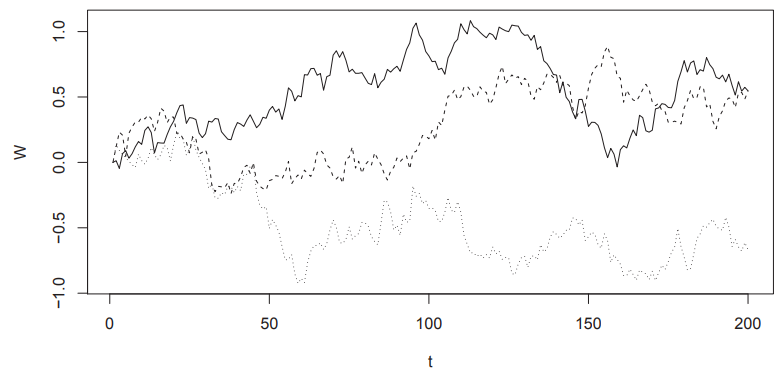
\includegraphics[height=7cm]{gb/K1G3.png}
    \caption{Simulasi Gerak Brown.}
    \label{K1G3}
\end{figure}

\begin{figure}
    \centering
    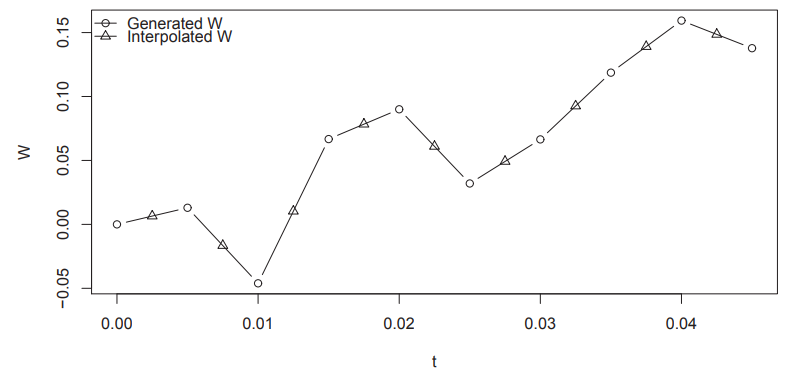
\includegraphics[height=7cm]{gb/K1G4.png}
    \caption{Interpolasi Gerak Brown.}
    \label{K1G4}
\end{figure}



\section{Latihan}





\newpage
\printbibliography[heading=bibintoc,title={Daftar Pustaka}]

\end{document}
